\documentclass{article}
\usepackage{graphicx}
\usepackage{float}

\begin{document}

\title{Tarea 4}
\author{Mauricio Neira - 201424001}

\maketitle

Este documento presenta los resultados de la tarea 4 de metodos computacionales. Fue desarrollado tomando $v = 1$, $dt = 0.025s$, $dx = 1cm$. \\

A continuacion se presentan los resultados concretos:

\section{Temperatura de la placa}
\subsection{Condiciones de frotera ABIERTAS}
\subsubsection{$100^\circ C$ constante}
\begin{figure}[H]
\minipage{0.32\textwidth}
  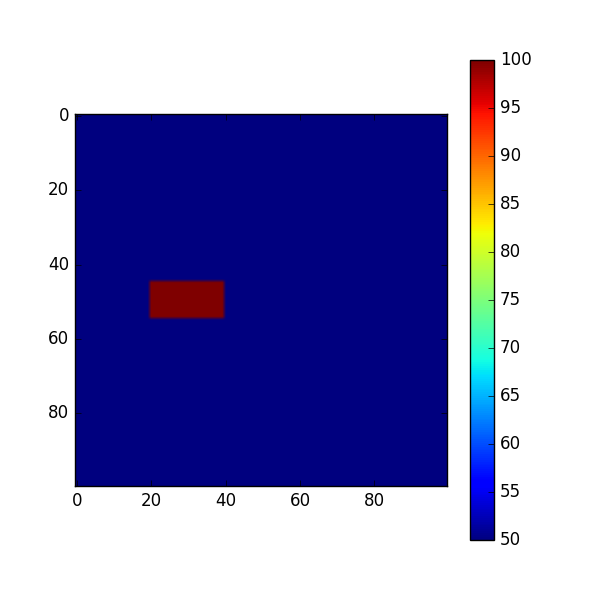
\includegraphics[width=\linewidth]{abiertasCte0.png}
  \caption{t =0s}\label{fig:awesome_image1}
\endminipage\hfill
\minipage{0.32\textwidth}
  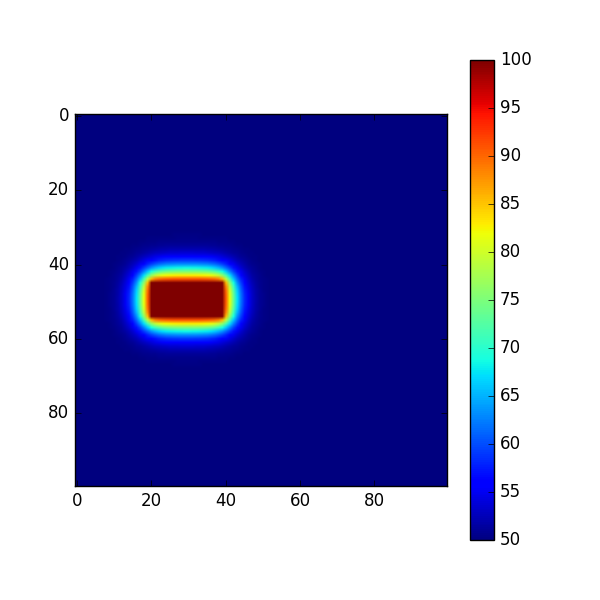
\includegraphics[width=\linewidth]{abiertasCte100.png}
  \caption{t = 100s}\label{fig:awesome_image2}
\endminipage\hfill
\minipage{0.32\textwidth}%
  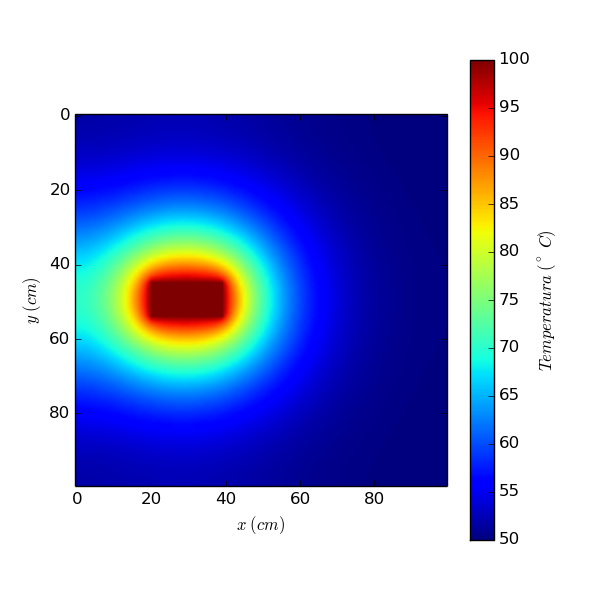
\includegraphics[width=\linewidth]{abiertasCte2500.png}
  \caption{t = 2500s}\label{fig:awesome_image3}
\endminipage
\end{figure}



\subsubsection{$100^\circ C$ NO constante}

\begin{figure}[H]
\minipage{0.32\textwidth}
  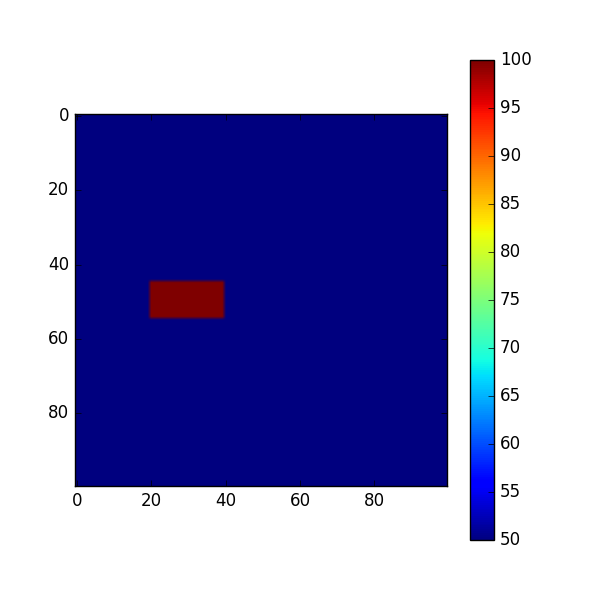
\includegraphics[width=\linewidth]{abiertasNOCte0.png}
  \caption{t =0s}\label{fig:awesome_image1}
\endminipage\hfill
\minipage{0.32\textwidth}
  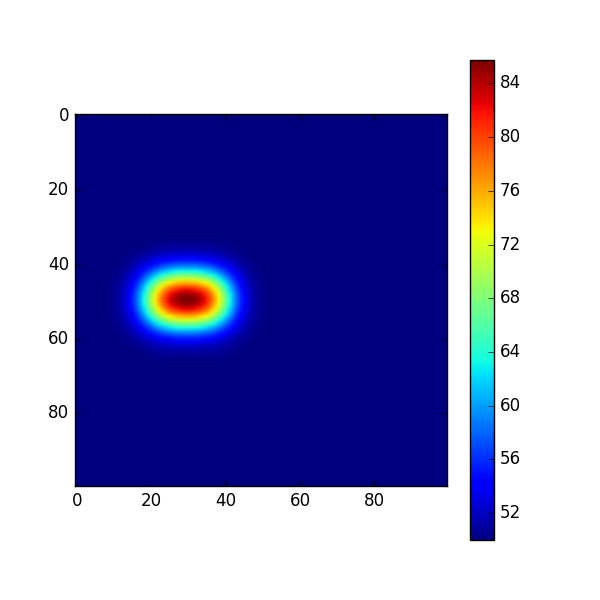
\includegraphics[width=\linewidth]{abiertasNOCte100.png}
  \caption{t = 100s}\label{fig:awesome_image2}
\endminipage\hfill
\minipage{0.32\textwidth}%
  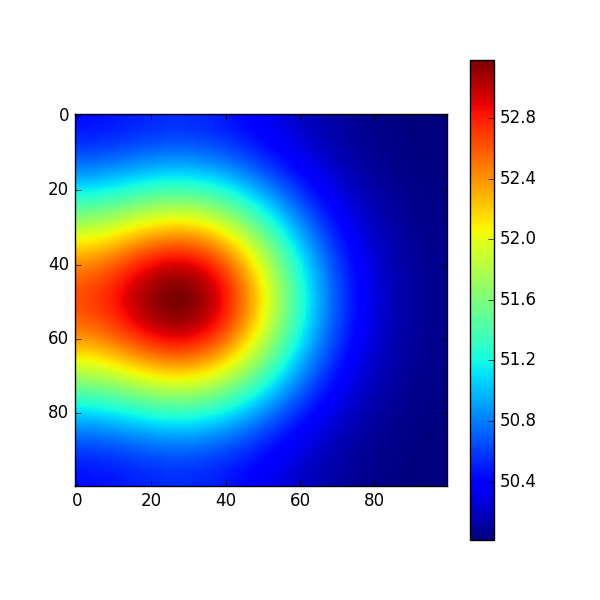
\includegraphics[width=\linewidth]{abiertasNOCte2500.png}
  \caption{t = 2500s}\label{fig:awesome_image3}
\endminipage
\end{figure}



\subsection{Condiciones de frotera PERIODICAS}
\subsubsection{$100^\circ C$ constante}
\begin{figure}[H]
\minipage{0.32\textwidth}
  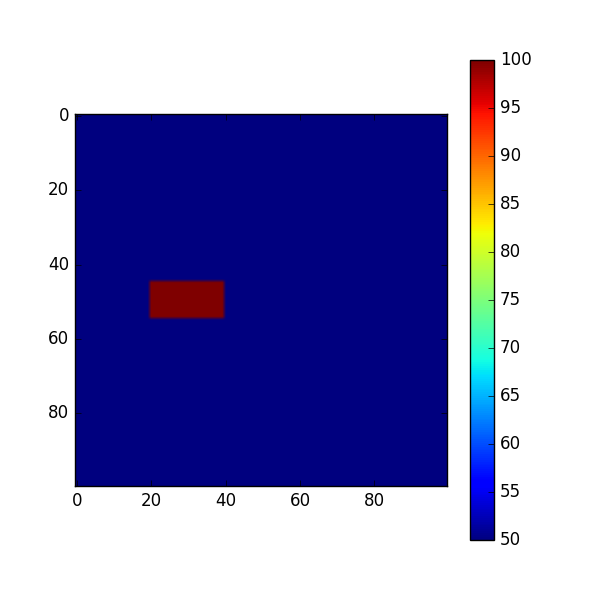
\includegraphics[width=\linewidth]{periodicasCte0.png}
  \caption{t =0s}\label{fig:awesome_image1}
\endminipage\hfill
\minipage{0.32\textwidth}
  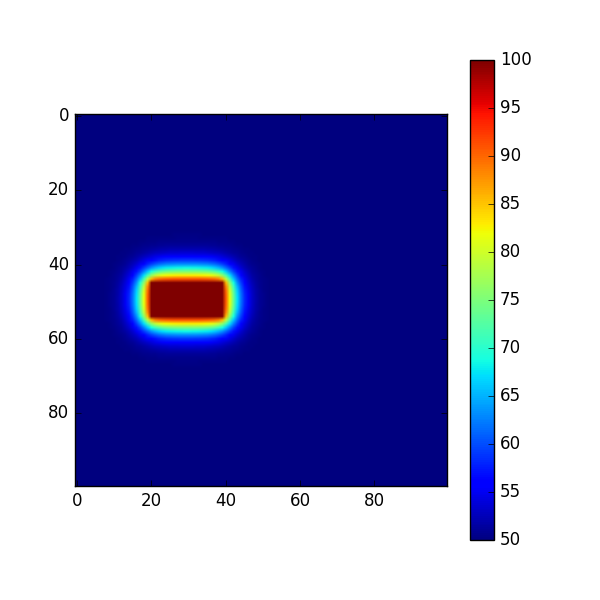
\includegraphics[width=\linewidth]{periodicasCte100.png}
  \caption{t = 100s}\label{fig:awesome_image2}
\endminipage\hfill
\minipage{0.32\textwidth}%
  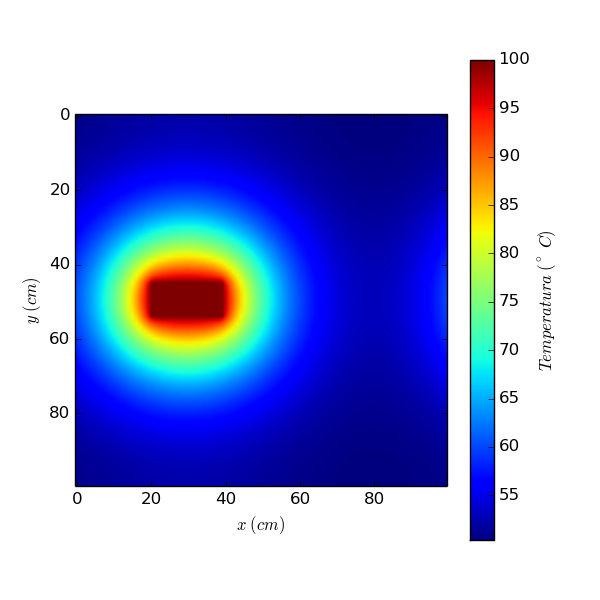
\includegraphics[width=\linewidth]{periodicasCte2500.png}
  \caption{t = 2500s}\label{fig:awesome_image3}
\endminipage
\end{figure}

\subsubsection{$100^\circ C$ NO constante}
\begin{figure}[H]
\minipage{0.32\textwidth}
  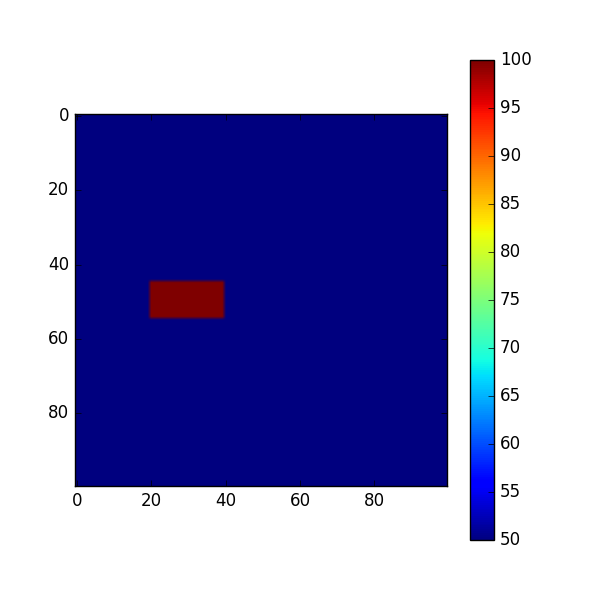
\includegraphics[width=\linewidth]{periodicasNOCte0.png}
  \caption{t =0s}\label{fig:awesome_image1}
\endminipage\hfill
\minipage{0.32\textwidth}
  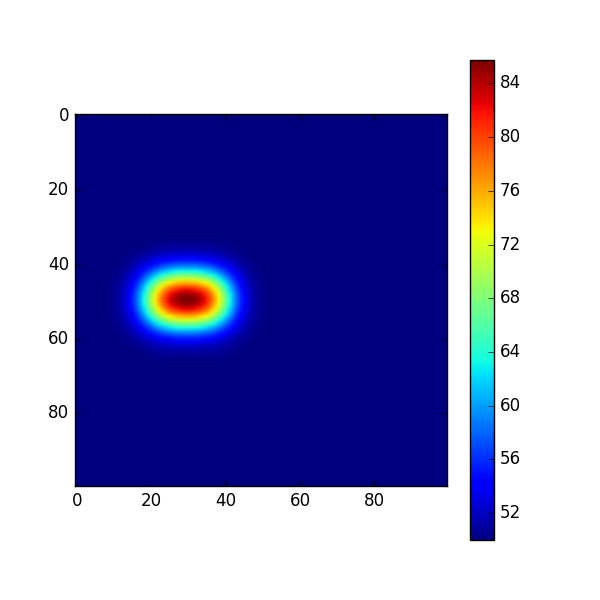
\includegraphics[width=\linewidth]{periodicasNOCte100.png}
  \caption{t = 100s}\label{fig:awesome_image2}
\endminipage\hfill
\minipage{0.32\textwidth}%
  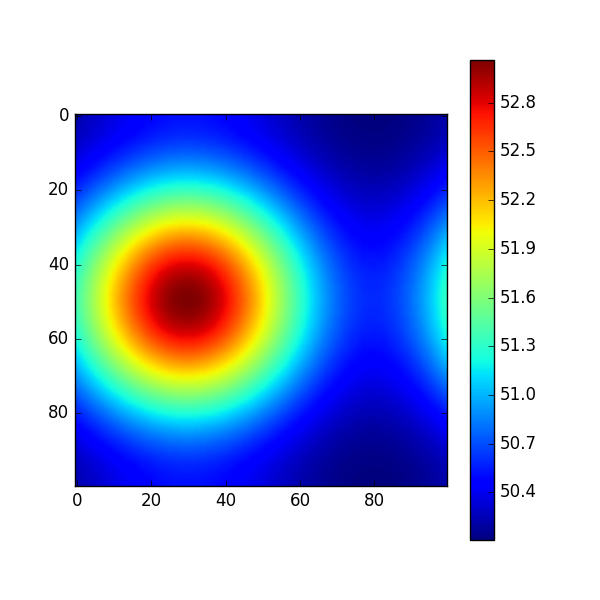
\includegraphics[width=\linewidth]{periodicasNOCte2500.png}
  \caption{t = 2500s}\label{fig:awesome_image3}
\endminipage
\end{figure}


\subsection{Condiciones de frotera FIJAS}
\subsubsection{$100^\circ C$ constante}
\begin{figure}[H]
\minipage{0.32\textwidth}
  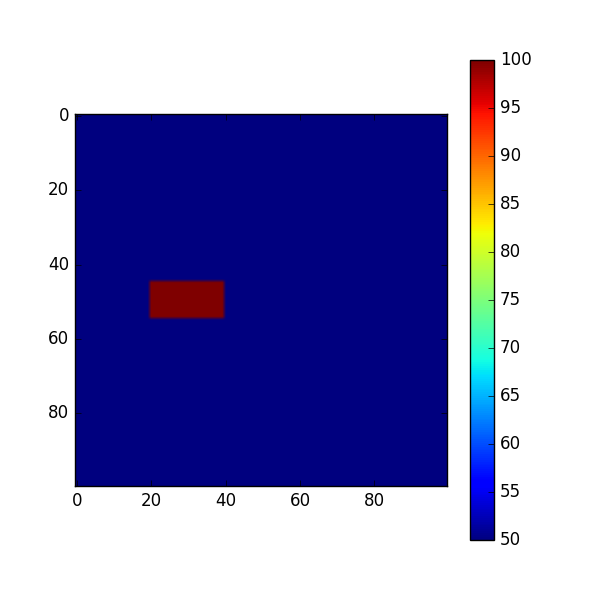
\includegraphics[width=\linewidth]{fijasCte0.png}
  \caption{t =0s}\label{fig:awesome_image1}
\endminipage\hfill
\minipage{0.32\textwidth}
  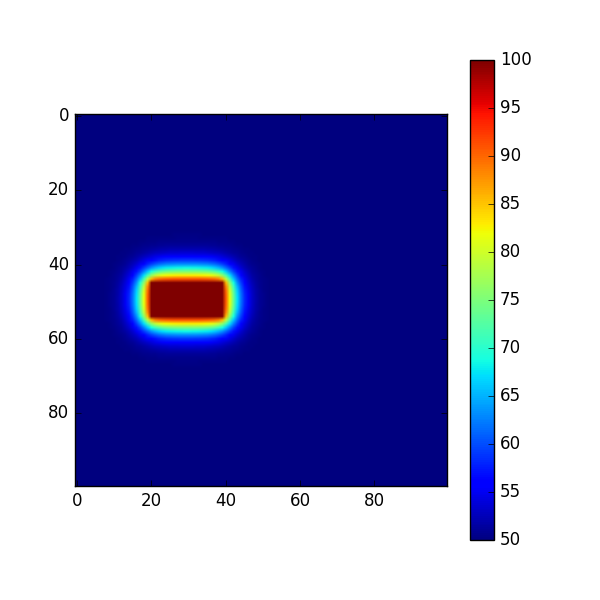
\includegraphics[width=\linewidth]{fijasCte100.png}
  \caption{t = 100s}\label{fig:awesome_image2}
\endminipage\hfill
\minipage{0.32\textwidth}%
  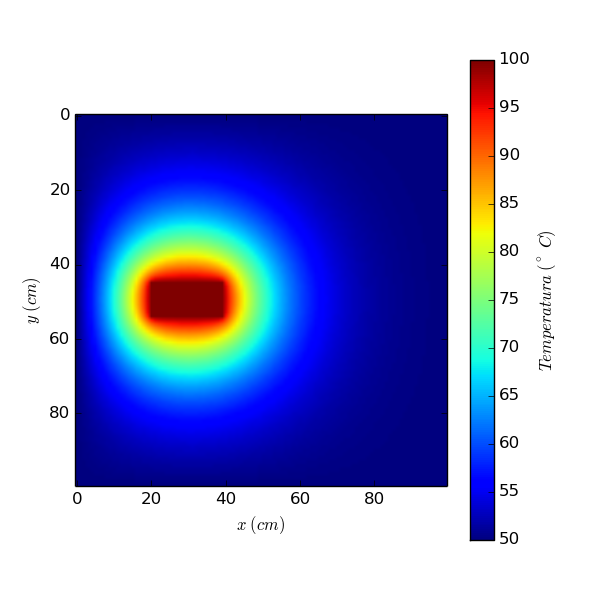
\includegraphics[width=\linewidth]{fijasCte2500.png}
  \caption{t = 2500s}\label{fig:awesome_image3}
\endminipage
\end{figure}

\subsubsection{$100^\circ C$ NO constante}
\begin{figure}[H]
\minipage{0.32\textwidth}
  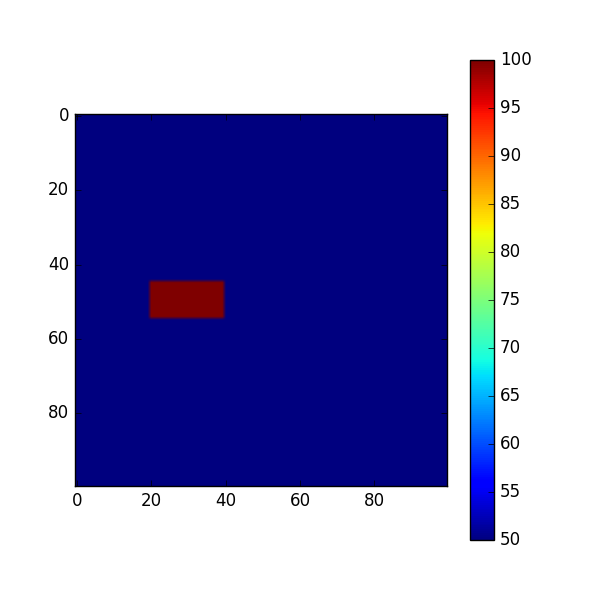
\includegraphics[width=\linewidth]{fijasNOCte0.png}
  \caption{t =0s}\label{fig:awesome_image1}
\endminipage\hfill
\minipage{0.32\textwidth}
  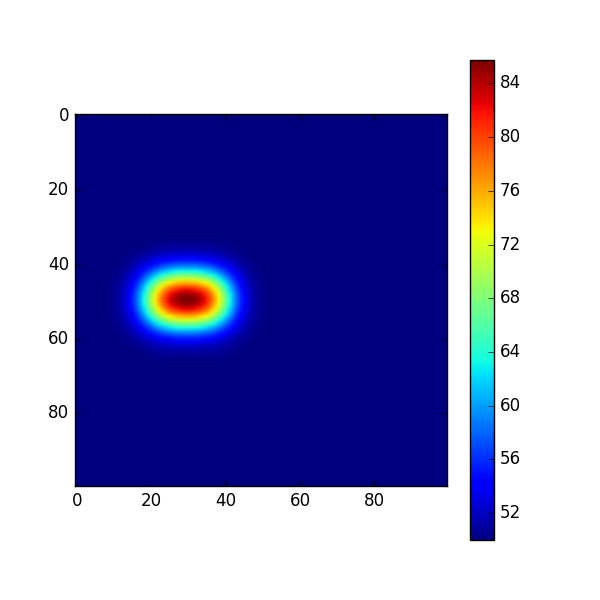
\includegraphics[width=\linewidth]{fijasNOCte100.png}
  \caption{t = 100s}\label{fig:awesome_image2}
\endminipage\hfill
\minipage{0.32\textwidth}%
  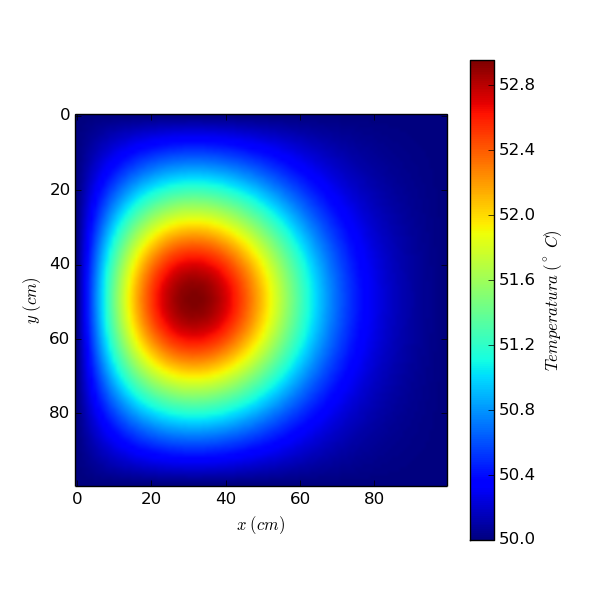
\includegraphics[width=\linewidth]{fijasNOCte2500.png}
  \caption{t = 2500s}\label{fig:awesome_image3}
\endminipage
\end{figure}


\section{Temperatura de promedio}
\subsubsection{$100^\circ C$ constante}

\begin{figure}[H]
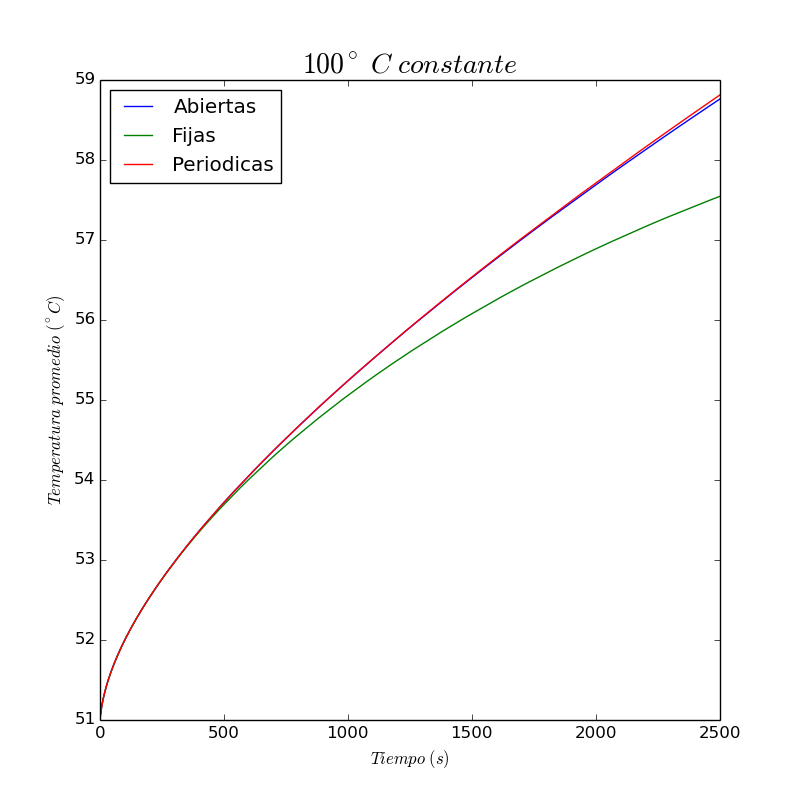
\includegraphics[width=\linewidth]{promCaso1.png}
\caption{Promedios de temperatura}
\end{figure}
\subsubsection{$100^\circ C$ NO constante}
\begin{figure}[H]
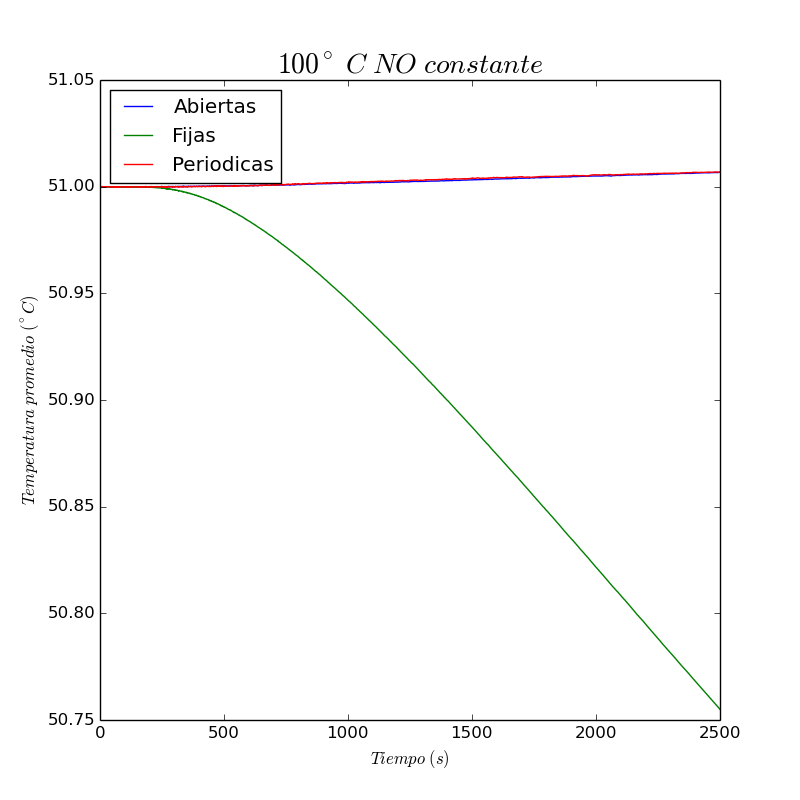
\includegraphics[width=\linewidth]{promCaso2.png}
\caption{Promedios de temperatura}
\end{figure}

\end{document}
